\section{カルシウムイメージングデータ}
本節では,カルシウムイメージングデータがどのようなデータなのかを説明し,どの程度の情報が取り出せるかを議論する.

ニューロンは1[ms]単位で活動電位が発生する(発火).
活動電位は細胞内外のイオン濃度が局所的に変化することによって生じる.
活動電位は細胞体から軸索を伝わり,シナプスを介して結合している別のニューロンに伝わる.
哺乳類の皮質ニューロンにおいて,ニューロンからニューロンへシナプスを介して活動電位が伝わるには数十[ms]かかる\cite{Izhikevich2004}.
このように活動電位を伝えることによってニューロン間で情報がやり取りされる.

ニューロンが他のニューロンとコネクションを持つ状態のことをコネクティビティという.
脳のコネクティビティには,anatomical connectivityとfunctional connectivityとeffective connectivityの3種類がある\cite{Sporns2007}.
Anatomical connectivityはニューロンが物理的に繋がっていることを指す.
Functional connectivityを持つ2つのニューロンは活動に相関があり,機能が同じことを指す.
例えば,ある物を見た時,それに特異的に反応するニューロン群はfunctional connectivityを持つ.
Effective connectivityは,1つのニューロンから別のニューロンへ情報が伝わることを指す.
脳の機能解明のためにはfunctional connectivityとeffective connectivityの推定が必要である.
脳内にはセルアセンブリというニューロン群が存在すると言われており\cite{Harris2012},セルアセンブリ内のニューロンはある刺激の元で同時に活動することが知られている.
セルアセンブリはfunctional connectivityを持っていると考えられるので,functional connectivityを推定することはセルアセンブリの推定につながる.
Effective connectivityは情報伝達の順番が分かるため,これも脳の機能解明につながる.
例えば,リアクチベーション現象があることが知られている.
リアクチベーション現象とは,ニューロンが同じ順番で発火することが繰り返されることであり,記憶の定着などにも関わっていると言われている.
データによってどのコネクティビティの情報を取り出せるかは異なり,電気生理ではeffective connectivityが推定できるが,サンプリングレートの低いカルシウムイメージングデータではfunctional connectivityまでしか推定ができない.

1個1個のニューロンを1[ms]単位で計測できればニューロン全ての活動を計測できるが,そのような技術は存在しない.
ニューロンの計測方法には様々なものがあり,それぞれ計測可能な時間分解能と空間分解能が異なる.
計測方法別の分解能については\cite{Sejnowski2014}のFig 1が分かりやすい.
EEG,PET,fMRIは脳の一部のニューロンの活動によって生じた電位,血流,代謝量の変化を計測する.
これらの手法ではニューロン単位の計測は行えないが,脳全体を計測することができる.
電気生理学的な手法やカルシウムイメージングではニューロン単位で膜電位の変化やカルシウムイオン濃度の変化を計測する.
これらの手法ではニューロン1個1個を計測できるが脳全体を計測することはできない.

カルシウムイメージングとはニューロン内のカルシウムイオン濃度を可視化することでニューロンの活動を計測する手法である.
観察したい個体のニューロンにカルシウムイオンと結合する蛍光タンパク質を発現させると,細胞内のカルシウムイオン濃度に応じて蛍光強度が変化する.
ニューロンが発火するとカルシウムイオンが流入するため蛍光強度が上昇し,その後徐々に蛍光強度は減少する.
ニューロンを蛍光顕微鏡で観察することで\Figref{fig:imagingB}のような蛍光強度を反映した画像が得られる.
その画像から個々のニューロンの蛍光強度のデータを取得できる.
\begin{figure}[htbp]
	\centering
	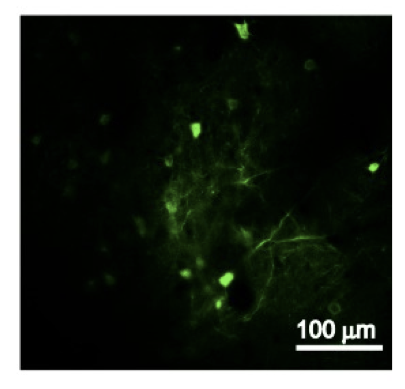
\includegraphics[width=0.5\hsize]{imagingB}
	\caption{カルシウムイメージングで観察できる画像の例.}
	\label{fig:imagingB}
\end{figure}

電気生理学的な手法と比べた時のカルシウムイメージングの利点として,ニューロンの位置情報が分かるため同じニューロンを複数回観察できることとより多くのニューロンの測定ができることが挙げられる.
また,ニューロンには興奮性ニューロンと抑制性ニューロンの二種類があり,カルシウムイメージングではこの種類を見分けることができる.
二種類の蛍光タンパク質を用いて,片方の蛍光タンパク質を抑制性ニューロンのみに発現させることで興奮性・抑制性が分かる.

カルシウムイメージングが電気生理学的な手法より劣る点として,時間分解能が挙げられる.
カルシウムイメージングのサンプリングレートは測定機器に限界があり\cite{Nakamura2003},通常1-50[Hz]程度である.
ニューロンの発火は約1[ms]で,シナプスを介して発火が伝わるのは40[ms]以内\cite{Bi1998}なので,ニューロンの発火を個別に観測することはできず,低いサンプリングレートでは発火の伝達も捉えることができない.
また,カルシウムイオン濃度の変化は発火のタイムスケールより長い.
発火後に蛍光強度が変化し始めるのは数[ms]後,蛍光強度がピークに達するのは数100[ms]後である.
一方,蛍光強度が元の値に戻るまでには,数100[ms]から数1000[ms]かかる\cite{Hira2018}.
また,蛍光タンパク質の性能によっても時間遅れが生じる.

本研究で扱うデータのサンプリングレートは8[Hz]で,シナプス伝達一つを見るには不十分である.
顕微鏡で観測すると活動電位が伝わる順番は分からなくなるため,カルシウムイメージングデータからはニューロンの活動の相関の情報しか得ることができない.
% また,脳の神経細胞はシナプスを3つか4つ介せば全て繋がると言われているため,局所的なネットワーク構造を考える必要はないと考えられる.
これより,このデータではニューロン間のシナプス伝達を推定するのではなく,機能的に同じニューロン,つまり同時に活動するニューロングループを推定する問題が適していると考えられる.
機能的に同じニューロンは,3つの脳のコネクティビティのうちfunctional connectivityで繋がっているニューロンを指す.
